\documentclass[times, utf8, zavrsni, english]{fer}
\usepackage{booktabs}
\usepackage{graphicx}
\graphicspath{ {./images/} }

\begin{document}

% TODO: Navedite broj rada.
\thesisnumber{000}

% TODO: Navedite naslov rada.
\title{Application of machine learning to threat classification from cybersecurity records}

% TODO: Navedite svoje ime i prezime.
\author{Mirta Medak}

\maketitle

% Ispis stranice s napomenom o umetanju izvornika rada. Uklonite naredbu \izvornik ako želite izbaciti tu stranicu.
\izvornik

% Dodavanje zahvale ili prazne stranice. Ako ne želite dodati zahvalu, naredbu ostavite radi prazne stranice.
\zahvala{}

\tableofcontents

\chapter{Introduction}
Every entity that is dependent on a computer system, from corporations to individuals, could be a subject to cyberattacks. \\
In 2018 there were 80,000 cyberattacks per day or over 30 million attacks per year. [1] During the CoVid-19 pandemic, cybercrime went up 600 \%, as PurpleSec suggests. [2] \\
As technology evolves, more various threats to its security emerge.
Tracking, describing, and evaluating these threats is of use when developing defense systems and making business decisions. \\

A \textbf{vulnerability} is a weakness in a computer system, that an attacker can exploit to execute malicious commands, access data in an unauthorized way, or perform other types of cyber attacks. [4,5] \\
A \textbf{threat} is any circumstance or event which has the potential to compromise system security. [6] \\
In order to tackle the cybersecurity problems in a more organized manner, a system of \emph{CVE (Common Vulnerability and Exposure)} has been developed. \\
The \emph{MITRE Corporation} maintains a public database of an increasing number of CVE records. \\
A CVE record includes an ID, a brief description of the vulnerability, and references.

In order to manipulate and prioritize vulnerabilities in a system, the metric of the Common Vulnerability Scoring System (CVSS) score is used. This metric estimates how "dangerous" exploitation of a vulnerability is. CVSS is an emerging standard of vulnerability comparison. [8] \\
CVSS is divided in three groups: \emph{Base, Temporal and Environmental score}. 
\textbf{Base Score} group shows the traits of the vulnerability that do not change over time and are not dependent on the environment. [9] Predicting the base score will be the subject of this research. \\

\begin{figure}[h]
	\caption{There are eight CVSS Base submetrics:}
	\centering
	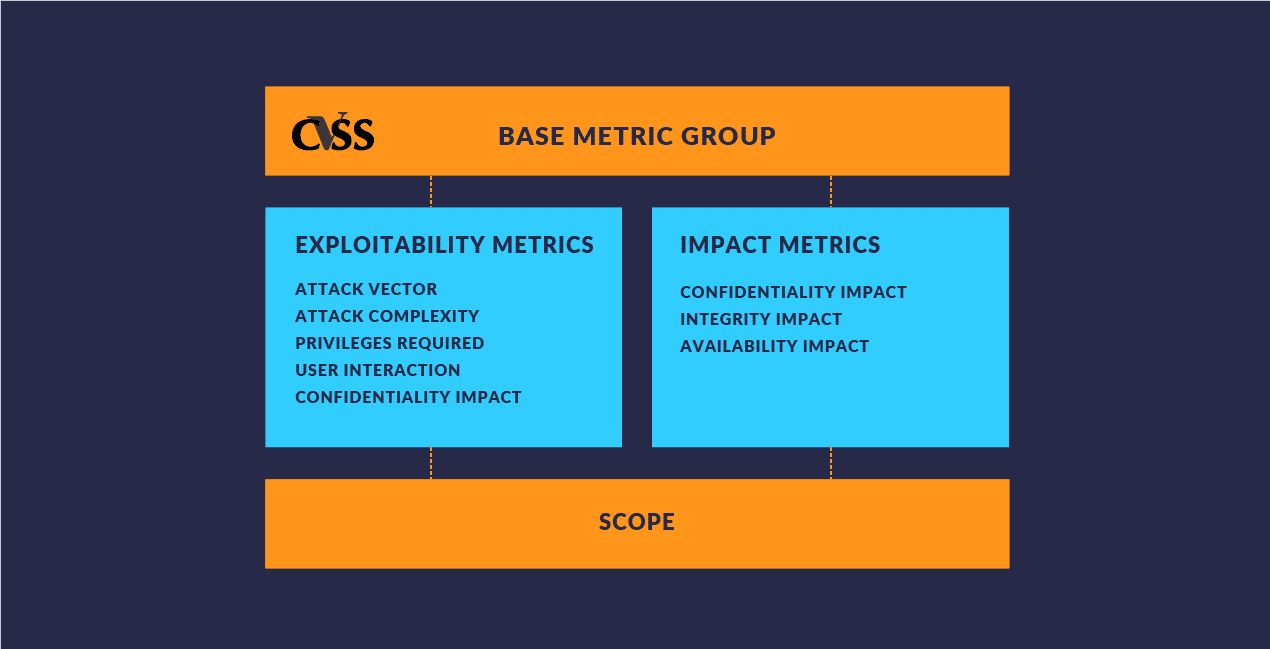
\includegraphics[scale=0.25]{CVSS-Base-Metric-Group}
\end{figure}
Each submetric is assigned by experts. E. g., attack complexity can be assigned as High or Low. The submetrics values all add a different weight to the score. This ratio of how much each submetric matters, is decided by engineers. This formula is then used to compute the score. [Bozorgi et al.] \\
Atefeh Khazaei et al. show an important concern in their work [8]: the CVSS calculation \textbf{can be subjective}.
Moreover, the annotation requires experts and time, which is prolonging the process and is costly. \\
Sometimes, all of the information needed to compute CVSS scores may not be available. Many vulnerabilities aren't assigned the score at all. [7, 10] \\
That is why it would be helpful if CVSS score is automatically decided based on the description of the vulnerability.

The goal of this research is to explore objective and automatic ways to obtain CVSS score. 
NLP methods are used to predict the CVSS Base score by analyzing the description from the CVE record. \\
BERT classification model has proven to be 90-95 \% accurate in predicting the submetrics using the description of the vulnerability. \\
BERT is computationally expensive, and sometimes it is advised to try simpler models first, because they might work just as well. That is why Support Vector Regression has been used to predict CVSS score from description too.

\chapter{Related work}
Inspiration to do this research has been given by the study of Cook, Bryan, et al., who have developed an application that takes any vulnerability description and gives its CVSS score. [10] They used BERT classification to predict the Base score submetrics. The CVSS score was then calculated using the hard-coded CVSS formula and the predicted submetrics results. They have achieved accuracy in the 0.90 range. \\

Another study developing an objective method of CVSS score calculation, written by Khazaei et al. [], used Support Vector Machine, Random-Forest, and fuzzy system. Their model's accuracy was around 0.86. \\

This problem was approached in detail by Bozorgi et al. [] Instead of predicting the CVSS score itself, they have developed a new classification system, using various features of the vulnerability. \\

\chapter{Data}
\section{Data acquisition}
Dataset used has been acquired and prepared by Cook et al., when used in their work \emph{Using NLP to Predict the Severity of Cybersecurity Vulnerabilities, 2021.}
Most of the data is publicly available and maintained by the MITRE organization and the National Institute of Standards of Technology. \\
From the cited research, we find out that at the beginning of 2021, only 50 \% of CVE records had a CVSS score assigned. \\
The datasets were created by human experts and therefore didn't require much preparation or preprocessing. 

\section{Dataset structure}
The entire dataset counts 77,020 entries. It is split into training set (80\%) and test set (20\%).

\begin{table}[h!]
	\centering
	\begin{tabular}{||c c c ||} 
		\hline
		 & Column Title & Values  \\ [0.5ex] 
		\hline\hline
		
		1 & attack\_vector & physical; adj\_network;   \\
		 & &  local; network \\
		2 & attack\_complexity & high; low  \\
		3 & privileges\_required & high; low; none  \\
		4 & user\_interaction & none; required \\ 
		5 & scope & unchanged; changed \\ 
		6 & confidentiality & high; low; none  \\
		7 & integrity & high; low; none  \\
		8 & availability & high; low; none  \\
		
		\hline\hline
		9 & description & natural language description \\
		10 & base\_score & float from 0 - 10 \\
		\hline
	\end{tabular}
\caption{Columns and their values used in experiments}
\label{table:1}
\end{table}

The first eight entries of Table 3.1. correspond to eight submetrics of CVSS base score.
\section{Dataset analysis}
According to CVSS v3.0 Ratings [nistgovstranica] the severity is classified in the following ranges:
\begin{table}[h!]
	\centering
	\begin{tabular}{| c c c ||} 
		\hline
		Severity & Base score range & No. of examples\\ [0.5ex] 
		\hline\hline
		
		None & 0.0 & 0  \\
		Low &  0.1-3.9 & 1115 \\
		Medium & 4.0-6.9 & 24232  \\
		High & 7.0-8.9  & 26793 \\
		Critical & 9.0-10.0 & 9476\\
		\hline
	\end{tabular}
	\caption{CVSS range classification and number of examples in each class (from the training set)}
	\label{table:2}
\end{table}
From Table 2. we can clearly see that the medium to high scores prevail. 

\chapter{Models}

\section{Support Vector Regression}
\subsection{Support Vector Machines}
The Support Vector algorithm was developed in its present form at AT\&T Bell Laboratories by Vapnik with colleagues. [11,12] \\

The Support Vector Machines are supervised learning models, that can be applied to classification, regression, and outliers detection problems. [13] \\
In classification problems, the output is a discrete variable, and in regression it is continuous. \\
The SV algorithm needs to find a function in n-dimensional space which fits the data. 
Support Vectors are the data points around this function. A flexible tube is formed symmetrically around the function so that the absolute values of errors less than a certain threshold are ignored both above and below the estimate. This way, the data points outside of the tube are penalized, and those on the inside are not. [14] \\
The SVR tries to find the narrowest tube centered around the function while minimizing the prediction error. [15] \\

The advantage of SVR is that its complexity does not depend on the dimension of the input space. [14] \\

Depending on the choice of kernel, data is mapped into different dimensional spaces. Kernel functions can be linear, rbf, polynomial, and sigmoid. \\
The free parameters of the model are C and epsilon. \\
The model is defined by its hyperparameters. They control the way the model fits the data. Their fine-tuning was performed using Bayesian optimization, which is based on the Bayesian theorem. More commonly used Grid Search tries out all given combinations of parameters. Bayes Search, as opposed to Grid Search, memorizes the result of the previous combination and uses it to choose the next combination, so that it comes to the optimum more quickly. [16] \\

The SVR, as well as other Support Vector models that will be mentioned, are implemented using scikit learn library. Implementation details are described in Chapter 5. Experiments and Results.

\subsection{word2vec}
Word2vec is a way to represent natural language as vectors. It was developed by Mikolov et al. in 2013. [17] \\
It consists of two learning models: Continuous Bag of Words (CBOW) and Skip-gram. CBOW predicts the word given its context, and Skip-gram predicts the context given a word. [18] \\
Knowing the distances between vectors, it is possible to group similar words.
This algorithm is used to convert the text input into vectors, after which they can be used in Support Vector Regression tasks.
\subsection{LinearSVR and SGDRegressor}
LinearSVR is similar to a Support Vector Regression model with a linear kernel. 
The difference is that LinearSVR is implemented as a liblinear model, and SVR as libsvm. [scikit learn] \\
SGD stands for Stochastic Gradient Descent. This is an iterative method of finding a function optimum. The gradient of the loss is estimated each sample at a time and the model is updated along the way with a decreasing learning rate. [scikit learn] \\
It is advised to use LinearSVR or SGDRegressor over SVR for large datasets. [scikit learn] 

\section{BERT}
\subsection{BERT architecture}
\textbf{Bidirectional Encoder Representations from Transformers} is a fairly new and revolutionary language representation model, developed by Google (Delvin et al. 2018) [20]. \\
BERT is fundamentally a transformer language model.
Developed by Vaswani et al., 2017, the \textbf{Transformer} is a network architecture based on attention mechanisms. Until the invention of transformers, more complicated models such as recurrent and convolutional neural networks with an encoder and a decoder were used to solve translation tasks. The new model improved translation, sequence modeling, and other similar tasks. [21] \\
The transformer architecture is based on an encoder that maps an input to a continuous representation, and a decoder that produces the output using the encoded representation, one element at a time. At every step, the model takes into account the previously encoded symbols by including them in the input. This way, the model considers the context. [21] \\
By definition, an attention function is mapping vectors as a weighted sum to an output, where the vectors correspond to a query, keys, and values. \\
The novelty in the BERT model is the bidirectional encoder, that is, the incorporation of context from both directions. This matters significantly in token-level tasks, such as question answering, token classification, etc. In order to perform bidirectional pre-training, BERT uses masked language models. [20] \\
A great advantage of BERT over other language models is that the model has been already pre-trained on large text corpora. This model can then be fine-tuned with only one more output layer, and this model can be applied to a variety of tasks. [20] This framework is called transfer learning. \\
When implementing BERT to a specific task, we can use an already pre-trained model. Our task is then to fine-tune it.
Fine-tuning is in fact putting data through a transformer self-attention mechanism.
\subsection{Data prepartion for BERT}
The dataset has to be split into train, development, and test set.\\
Attributes that are necessary to fine-tune BERT are the following:
\begin{itemize}
	\item input ids - list of tokens, smallest units of text that make sense,
	\item  input mask - implies that all sequences that are longer than a specified length of a sequence will be truncated to that specified length, and those that are shorter will be padded with additional tokens,
	\item label id - id of the label for a sequence.
\end{itemize}
 
\subsection{BERT classification}
As previously mentioned, in order to fine-tune BERT for a specific task, an additional task-related output layer is added to an already pre-trained model.\\
In this research, the \texttt{bert-base-uncased} was used as the pre-trained model.\\
Some common tasks are implemented in the transformers library as the top layer. One of those is BertForSequenceClassification, which was used in this research to predict the eight submetrics of the Base score. 
\subsection{BERT for regression}
Similarly to the classification task, on top of 12 transformers lies a BertRegressor layer that gives the output for a regression task. The Bert Regressor was used to predict the base score directly from the description.\\
BERT Regressor is widely used in machine translation evaluation tasks. [22]

\chapter{Experiments and results}
\section{Base score prediction from vulnerability description}
The goal of this experiment was to find out if it is possible to accurately obtain the CVSS score by direct analysis of the vulnerability description.
\subsection{Support Vector Regression + word2vec}
The dataset of over 61k entries is too large for the Support Vector Regression model implemented as \texttt{libsvm}, because the fit complexity is more than quadratic with the number of samples.\\
That is why SVR used approximately half of the training data, 30k samples, and 6k test samples. 
10k samples were used to fine-tune the hyperparameters. \\
All samples taken from the initial dataset were stratified with regard to the Base score, that is, the data was chosen in such a way, that the Base score values follow a uniform distribution.\\
Vulnerability description tokens are transformed into vectors and then summarized in order to map one vector to one description.
These vectors are then scaled using the StandardScaler's function .fit\_transform(X,y), which first fits the input data to the output feature, and then scales it.\\
Parameter fine-tuning is then performed by BayesSearchCV, the function from \texttt{skopt} library. The kernel was set to rbf, because the SVR linear kernel is too slow for large datasets.\\
Bayes Search optimized the following hyperparameters:
\begin{table}[h!]
	\parbox{.45\linewidth}{
	\centering
	
	\begin{tabular}{|| c | c ||} 
		\hline
		Parameter & Value \\ [0.5ex] 
		\hline\hline
		C & 31.6668  \\ \hline
		epsilon & 0.732095 \\ \hline
		tol & 0.003125  \\ 
		\hline
	\end{tabular}
	\caption{Hyperparameteres for SVR}
	\label{table:3}
}
	\parbox{.45\linewidth}{
	\centering
	\begin{tabular}{|| c | c ||} 
		\hline
		Metric & Value \\ [0.5ex] 
		\hline\hline
		Mean Squared Error & 1.711  \\ \hline
		Explained Variance Score & 0.504\\ \hline
		Maximum Residual Error & 6.186 \\ \hline
		Mean Absolute Percentage Error & 0.167 \\ \hline
		Coefficient of Determination (\textbf{R2 Score}) & \textbf{0.503} \\
		\hline
	\end{tabular}
	\caption{SVR results}
	\label{table:4}
}
\end{table}
\subsection{Linear Support Vector Regression}
Linear SVR used the entire dataset. \\
Again, the BayesSearchCV was used to optimize the hyperparameters.\\
Because the number of samples was greater than the number of features, the loss function had to be set as 'squared\_epsilon\_insensitive'.
\begin{table}[h!]
	\parbox{.45\linewidth}{
		\centering
		\begin{tabular}{|| c | c ||} 
			\hline
			Parameter & Value \\ [0.5ex] 
			\hline\hline
			C & 0.065189  \\ \hline
			epsilon & 2.1582e-06 \\ \hline
			tol & 0.00015387  \\ 
			\hline
		\end{tabular}
		\caption{Hyperparameteres for LinearSVR}
		\label{table:5}
	}
	\parbox{.45\linewidth}{
		\centering
		\begin{tabular}{|| c | c ||} 
			\hline
			Metric & Value \\ [0.5ex] 
			\hline\hline
			Mean Squared Error & 1.888  \\ \hline
			Explained Variance Score & 0.302\\ \hline
			Maximum Residual Error & 9.786 \\ \hline
			Mean Absolute Percentage Error & 0.169 \\ \hline
			Coefficient of Determination (\textbf{R2 Score}) & \textbf{0.302} \\
			\hline
		\end{tabular}
		\caption{LinearSVR results}
		\label{table:6}
	}
\end{table}
\subsection{Stochastic Gradient Descent Regressor}
SGDRegressor used the entire dataset as well. \\
Bayes Search optimized the hyperparameteres:
\begin{table}[h!]
	\parbox{.45\linewidth}{
		\centering
		\begin{tabular}{|| c | c ||} 
			\hline
			Parameter & Value \\ [0.5ex] 
			\hline\hline
			alpha & 5.1431e-05  \\ \hline
			epsilon & 0.37136 \\ \hline
			loss & "huber" \\ \hline
			tol & 1.5939e-07  \\ 
			\hline
		\end{tabular}
		\caption{Hyperparameteres for SGDRegressor}
		\label{table:7}
	}
	\parbox{.45\linewidth}{
		\centering
		\begin{tabular}{|| c | c ||} 
			\hline
			Metric & Value \\ [0.5ex] 
			\hline\hline
			Mean Squared Error & 1.952  \\ \hline
			Explained Variance Score & 0.279\\ \hline
			Maximum Residual Error & 9.786 \\ \hline
			Mean Absolute Percentage Error & 0.169 \\ \hline
			Coefficient of Determination (\textbf{R2 Score}) & \textbf{0.278} \\
			\hline
		\end{tabular}
		\caption{SGDRegressor results}
		\label{table:8}
	}
\end{table}
\subsection{BERT Regressor}
The BERT fine-tuning was done with PyTorch.\\
The library \texttt{transformers} is used to import the tokenizer and BertModel in order to create a class BertRegressor.
Firstly, the descriptions are tokenized using BertTokenizer. Then, the longest description is found. Using the method tokenizer.encode\_plus(), input\_ids and attention\_masks lists are created. Those lists, as well as the labels list, are converted into tensors. \\
The training dataset is split into 80-20 train-validation sets. \\
The optimizer used is AdamW with default parameters, and the scheduler is obtained with the function get\_linear\_schedule\_with\_warmup. 
The loss function is MSELoss.\\
The model was trained for three epochs. 

\begin{table}[h!]
		\centering
		\begin{tabular}{|| c | c ||} 
			\hline
			Metric & Value \\ [0.5ex] 
			\hline\hline
			Mean Squared Error & 1.186  \\ \hline
			Explained Variance Score & 0.563\\ \hline
			Maximum Residual Error & 6.953 \\ \hline
			Mean Absolute Percentage Error & 0.116 \\ \hline
			Coefficient of Determination (\textbf{R2 Score}) & \textbf{0.561} \\
			\hline
		\end{tabular}
		\caption{BERT regressor results}
		\label{table:9}
\end{table}
\subsection{Results comparison}
\begin{table}[h!]
	\centering
	\begin{tabular}{|| c | c ||} 
		\hline
		Model & R2 score \\ [0.5ex] 
		\hline\hline
		SVR & 0.503  \\ \hline
		LinearSVR & 0.302 \\ \hline
		SGDRegressor & 0.278 \\ \hline
		\textbf{BERT Regressor} & \textbf{0.561} \\ 
	
		\hline
	\end{tabular}
	\caption{Models comparison}
	\label{table:10}
\end{table}

\section{Base score submetrics classification}
The goal of this experiment was to discover at what level of accuracy can we predict the submetrics of the Base score, having the vulnerability description as the input.
\subsection{Baseline}
The Support Vector Classifier with default parameters was used as a baseline model for this prediction.\\
The description tokens were converted into vectors, and the vectors were summarized just like in SVR.\\

\subsection{BERT Classification}
The fine-tuning was performed with PyTorch.
Firstly, the dataset was divided into a test set (20\%) and the rest set, which was divided into a training set (80\%) and a development set.\\
From the \texttt{transformers} library, BertForSequenceClassification made up the top layer of the BERT model.\\
In the function \texttt{convert\_examples\_to\_inputs}\textit{(X, y, label2idx, max\_seq\_len, tokenizer)}, a list of token ids, segment ids, and input mask lists were created. Longer descriptions than max\_seq\_len were truncated, while the shorter ones were padded. \\
Usually, batch size is 16 or 32, in this model the value of batch size is 16.
The AdamW optimizer with a base learning rate of 5e-5  is used. The WarmupLinearScheduler linearly increases the learning rate during the warmup stage. During the training, the learning rate slowly decreases again.\\
The model was trained for three epochs.
At each epoch, the model is trained on the training set and evaluated on the development set. \\
To perform the final evaluation, the model is given test data that has never been seen before, and it predicts the submetric values.

\subsection{Results comparison}
\begin{table}[h!]
	\centering
	\begin{tabular}{|| c | c ||} 
		\hline
		Model & R2 score \\ [0.5ex] 
		\hline\hline
		SVR & 0.503  \\ \hline
		LinearSVR & 0.302 \\ \hline
		SGDRegressor & 0.278 \\ \hline
		\textbf{BERT Regressor} & \textbf{0.561} \\ 
		
		\hline
	\end{tabular}
	\caption{Models comparison}
	\label{table:10}
\end{table}
\chapter{Conclusion}
No system is without an error. As long as there is a flaw in the system, there exists a threat. The number of various flaws and threats continues to grow. This problem was systematically approached by MITRE and NIST, which maintain the database of Common Vulnerability and Exposure (CVE) records. Only a part of the records have been assigned their severity ranking, Common Vulnerability Scoring System (CVSS) score. This score helps in the risk assessment of the vulnerability. The CVSS base score is a result of eight submetrics, the values of which are assigned by human experts. Computing a CVSS score is a long and costly process, and it can be subjective. \\

In this research, more objective ways to get the CVSS score have been examined. Natural language processing methods were used to predict the CVSS base score directly from the vulnerability description.\\
Support Vector Regression and Bert Regressor have achieved the best results in this experiment, having the coefficients of determination R2(SVR) = 0.503 and R2(Bert) = 0.561. This implies that even the best models were not very accurate, and modifications ought to be done. Due to computational complexity, the training of both models lasted for a long time. \\
If the direct prediction does not work accurately, it is possible to predict the base score submetrics. Depending on the values of the submetrics the base score is calculated. The Support Vector Classifier was used as a baseline model. We can see the accuracy of 85-90 \%. BERT Sequence Classifier proved to be 90-95 \% accurate in these predictions. The conclusion is that we can use even less computationally expensive models, such as SVC, to achieve a high degree of accuracy in this task.\\
Compared to Vulnerwatch results...\\

Different models approach text tokens differently, so it is not clear in which way the text should be preprocessed. 
In order to achieve better models, the descriptions should be preprocessed in many different ways, and results should be compared.
An increase in the number of epochs in the BERT Regressor could make the result more accurate. 
\bibliography{literatura.bib}
\bibliographystyle{plainnat}


\listoffigures
\begin{abstract}
Abstract.

\keywords{Keywords.}
\end{abstract}

\hrtitle{Primjena strojnog učenja za klasifikaciju prijetnji iz zapisa o kibernetičkoj sigurnosti}
\begin{sazetak}
Sažetak na hrvatskom jeziku.

\kljucnerijeci{Ključne riječi, odvojene zarezima.}
\end{sazetak}

\end{document}
